\documentclass[12pt,a4paper,twoside]{article}
%
% default format and packages for pdflatex
%
% counteract default shifts of printers
\setlength{\hoffset}{-1.in}
\setlength{\voffset}{-1.in}
\setlength{\topmargin}{2.5cm}
\setlength{\headheight}{0.1cm}
\setlength{\headsep}{0.1cm}
\setlength{\textheight}{23.5cm}
\setlength{\textwidth}{16.cm}
\setlength{\oddsidemargin}{2.5cm}
\setlength{\evensidemargin}{2.5cm}
\pagestyle{empty}
%
% additional packages
%
\usepackage{amsmath,amssymb}
\usepackage[english]{babel}
\usepackage{color}
\usepackage{graphicx}
\usepackage{mathpazo}
\usepackage{palatino}
%\DeclareGraphicsExtensions{.eps,.jpg,.pdf,.png,}
\graphicspath{{./eps},{./pdf},{./png},{./jpg}} % Note, the additional {} are mandatory!
\usepackage[plainpages=false,pdfpagelabels]{hyperref}
\usepackage{psfrag}
\usepackage{xspace}

%%% Local Variables:
%%% mode: latex
%%% TeX-master: t
%%% End:

% Abk"urzungen
\def\R{{\mathbb{R}}}
\def\C{{\mathbb{C}}}
\def\N{{\mathbb{N}}}
\def\Z{{\mathbb{Z}}}
\def\Q{{\mathbb{Q}}}
\newcommand{\floor}[1]{{\lfloor #1\rfloor}}
\newcommand{\ceil}[1]{{\lceil #1\rceil}}

\newcommand{\braOket}[3]{\big\langle\,#1\,\big|\,#2\,\big|
  \,#3\,\big\rangle}
\newcommand{\ket}[1]{\left|\,#1\,\right\rangle}
\newcommand{\dd}{\mathrm{d}}

%
% Additional commands for numeration and table settings
%
%\renewcommand{\labelenumi}{{\bf \alph{enumi})}}
\providecommand{\hftwo}{\hspace*{\fill}}
\providecommand{\rbthm}{\rule[-2ex]{0ex}{5ex}}
\providecommand{\rbthr}{\rule[-1.7ex]{0ex}{5ex}}
\providecommand{\rbtrm}{\rule[-2ex]{0ex}{5ex}}
\providecommand{\rbtrr}{\rule[-0.8ex]{0ex}{3.2ex}}
\newcommand{\rmvec}[1]{{\rm \vec{#1}}}

%
% Measurements and units (base version from CMS PTDR)
%
\newcommand{\dg}{\ensuremath{^\circ}}
\newcommand{\ten}[1]{\ensuremath{\times {\rm 10}^{\rm #1}}}
\newcommand{\unit}[1]{\ensuremath{{\rm \,#1}}\xspace}
\newcommand{\mum}{\ensuremath{\,\mu{\rm m}}\xspace}
\newcommand{\micron}{\ensuremath{\,\mu{\rm m}}\xspace}
\newcommand{\cm}{\ensuremath{\,{\rm cm}}\xspace}
\newcommand{\mm}{\ensuremath{\,{\rm mm}}\xspace}
\newcommand{\mus}{\ensuremath{\,\mu{\rm s}}\xspace}
\newcommand{\volt}{\ensuremath{\,{\rm V}}\xspace}
\newcommand{\eV}{\ensuremath{\,{\rm e\hspace{-.08em}V}}\xspace}
\newcommand{\keV}{\ensuremath{\,{\rm ke\hspace{-.08em}V}}\xspace}
\newcommand{\MeV}{\ensuremath{\,{\rm Me\hspace{-.08em}V}}\xspace}
\newcommand{\GeV}{\ensuremath{\,{\rm Ge\hspace{-.08em}V}}\xspace}
\newcommand{\TeV}{\ensuremath{\,{\rm Te\hspace{-.08em}V}}\xspace}
\newcommand{\PeV}{\ensuremath{\,{\rm Pe\hspace{-.08em}V}}\xspace}
\newcommand{\keVc}{\ensuremath{{\,{\rm ke\hspace{-.08em}V\hspace{-0.16em}/\hspace{-0.08em}c}}}\xspace}
\newcommand{\MeVc}{\ensuremath{{\,{\rm Me\hspace{-.08em}V\hspace{-0.16em}/\hspace{-0.08em}c}}}\xspace}
\newcommand{\GeVc}{\ensuremath{{\,{\rm Ge\hspace{-.08em}V\hspace{-0.16em}/\hspace{-0.08em}c}}}\xspace}
\newcommand{\TeVc}{\ensuremath{{\,{\rm Te\hspace{-.08em}V\hspace{-0.16em}/\hspace{-0.08em}c}}}\xspace}
\newcommand{\keVcc}{\ensuremath{{\,{\rm ke\hspace{-.08em}V\hspace{-0.16em}/\hspace{-0.08em}c}^{\rm 2}}}\xspace}
\newcommand{\MeVcc}{\ensuremath{{\,{\rm Me\hspace{-.08em}V\hspace{-0.16em}/\hspace{-0.08em}c}^{\rm 2}}}\xspace}
\newcommand{\GeVcc}{\ensuremath{{\,{\rm Ge\hspace{-.08em}V\hspace{-0.16em}/\hspace{-0.08em}c}^{\rm 2}}}\xspace}
\newcommand{\TeVcc}{\ensuremath{{\,{\rm Te\hspace{-.08em}V\hspace{-0.16em}/\hspace{-0.08em}c}^{\rm 2}}}\xspace}
\newcommand{\pbinv} {\mbox{\ensuremath{\,{\rm pb}^{\rm $-$1}}}\xspace}
\newcommand{\fbinv} {\mbox{\ensuremath{\,{\rm fb}^{\rm $-$1}}}\xspace}
\newcommand{\nbinv} {\mbox{\ensuremath{\,{\rm nb}^{\rm $-$1}}}\xspace}
\newcommand{\percms}{\ensuremath{\,{\rm cm}^{\rm $-$2}\,{\rm s}^{\rm $-$1}}\xspace}
\newcommand{\lumi}{\ensuremath{\mathcal{L}}\xspace}
\newcommand{\Lumi}{\ensuremath{\mathcal{L}}\xspace}%both upper and lower

\providecommand{\FASTNLO}{{\textsc{fastNLO}}\xspace}
\providecommand{\NLOJETPP}{{\textsc{NLOJet++}}\xspace}

%%% Local Variables:
%%% mode: latex
%%% TeX-master: t
%%% End:

%
%
%
\begin{document}

\noindent{\bf Derivation of Scale and PDF Uncertainties and Comparison
  with
  Data for Jet Cross-Sections with \FASTNLO~\cite{Wobisch:2011ij}}\\

\noindent
Preparation:\\
This exercise can be performed with suitably, i.e. availability of
{\tt g++}/{\tt gfortran} compiler and LHAPDF library, prepared Linux
systems or with the virtual machine {\tt PDFLHC} that has been set up
for this PDF school. For performance reasons it is strongly
recommended, however, to attribute about 1 GB of memory to the VM
instead of just 1/2 GB\@. This can be done with {\tt virtualbox}
before starting up the VM\@. Otherwise compiling and linking might
become awfully slow.

Furthermore the following steps need to be carried out from within a
terminal session:

\begin{itemize}
\item[1.] Download the \FASTNLO reader software and one of the
  available \FASTNLO cross-section tables from the internet
  using {\tt wget} either from the indico page of today's tutorial\\
  \href{https://indico.desy.de/contributionDisplay.py?contribId=12&confId=6225}
  {https://indico.desy.de/contributionDisplay.py?contribId=12\&confId=6225}\\
  or from the fastNLO web page\\
  \href{http://fastnlo.hepforge.org/v21/code/fastnlo_reader-2.1.0-1273.tar.gz}{\tt
    http://fastnlo.hepforge.org/v21/code/fastnlo\_reader-2.1.0\\-1273.tar.gz}\\
  \href{http://fastnlo.hepforge.org/v21/tables/fnl1014_v2_all.tab.gz}{\tt
    http://fastnlo.hepforge.org/v21/tables/fnl1014\_v2\_all.tab.gz}
\item[2.] Decompress the \FASTNLO table\\
  {\tt  gunzip fnl1014\_v2\_all.tab.gz}\\
  and untar the archive of the reader program:\\
  {\tt tar xzvf fastnlo\_reader-2.1.0-1273.tar.gz}
\item[3.] Configure, compile, link and install the reader
  program:\\
  {\tt cd fastnlo\_reader-2.1.0-1273}\\
  {\tt ./configure --prefix=\$HOME}\\
  {\tt make}\\
  {\tt make install}
\item[4.] Test the produced executable:\\
  {\tt rehash}\\
  {\tt fnlo-cppread -h} $\rightarrow$ displays the usage and some options\\
  {\tt fnlo-cppread fnl1014\_v2\_all.tab} $\rightarrow$ prints the
  inclusive jet cross-sections corresponding to the CMS
  publication~\cite{CMS-PAP-QCD-10-011} with the default parton
  distributions (PDFs) according to CTEQ6M~\cite{Pumplin:2002vw}
  (cteq6m.LHpdf).
\item[5.] If this set is not available in the LHAPDF ({\bf L}es {\bf
    H}ouches {\bf A}ccord {\bf P}arton {\bf D}istribution {\bf
    F}unctions) installation of the VM, it and further ones
  can be downloaded from the LHAPDF projekt page~\cite{Whalley:2005nh}:\\
  {\tt lhapdf-getdata CT10.LHgrid}~\cite{Lai:2010vv}\\
  {\tt lhapdf-getdata NNPDF21\_100.LHgrid}~\cite{Ball:2011mu}\\
  {\tt fnlo-cppread fnl1014\_v2\_all.tab ./CT10.LHgrid} $\rightarrow$
  prints the inclusive jet cross-sections of CMS using the CT10 PDF
  set.
\end{itemize}

For a detailed evaluation as part of this tutorial you have to program
code in {\tt C++}\@. For this purpose you should read and edit the
elaborately commented main program code in {\tt fnlo-cppread.cc}
within the subdirectory {\tt reader\_cc}. Subsequently you have to
recompile and link via {\tt make; make install}.

\begin{enumerate}
\item Calculate the relative uncertainty of the jet cross-sections in
  next-to-leading order (NLO) when varying the renormalization and
  factorization scales $\mu_r$ and $\mu_f$ according to the six scale
  factor combinations (other than [1,1]) predefined in {\tt
    fnlo-cppread.cc}. A loop over these scale combinations has already
  been prepared within the code. Note that the uncertainty corresponds
  to the {\bf maximal} upward and downward deviations from the normal
  result.

\item Calculate the relative PDF uncertainty of the NLO jet
  cross-section using the Toy-MC-method required for the NNPDF~2.x
  PDFs. For this you have to program a loop over all replicas (members
  1 to 100) of the NNPDF~2.x PDFs.  The central result then is the
  average cross section and its uncertainty the {\bf
    $1\,\sigma$-standard deviation} of the resulting distribution of
  100 results (for each observable bin!).

  Note: As detailed in the example code {\tt fnlo-cppread.cc} the LO
  and NLO results for each observable bin can be accessed via:
\begin{verbatim}
    vector < double > xsnlo = fnloreader.GetCrossSection();
    vector < double > kfac  = fnloreader.GetKFactors();
    vector < double > xslo  = xsnlo;
    for (unsigned int i=0;i<xslo.size();i++){
      if ( abs(kfac[i]) > DBL_MIN ){
        xslo[i] = xslo[i]/kfac[i];
      } else {
        xslo[i] = -1.;
      }
    }
\end{verbatim}

  % \item Berechnen Sie die relative PDF Unsicherheit der NLO
  %   Jetwirkungsquerschnitte unter Verwendung der Eigenvektormethode
  %   mit den CT10 Partonverteilungen. Hierzu m\"ussen Sie eine
  %   Schleife \"uber alle PDF Variationen ({\it Members} 1 bis 52)
  %   der CT10 PDFs programmieren und jeweils die oberen und unteren
  %   Abweichungen vom Normalwert (Member 0) getrennt {\bf
  %     quadratisch} zum Gesamtfehler {\bf addieren}. Eine
  %   be\-stimm\-te PDF Datei kann \"uber\\ {\tt
  %     fnloreader->SetLHAPDFfilename(PDFFile);} und ein
  %   be\-stimm\-tes Mem\-ber darin \"uber\\ {\tt
  %     fnloreader->SetLHAPDFset(int PDFSet);} ausgew\"ahlt werden.

\item If you still have time you can also compare the calculated NLO
  cross sections with the data measured by the CMS Collaboration.
  They are contained in the table used for this tutorial and can be
  printed out via\\
  {\tt fnloreader->PrintCrossSectionsData();}.
\end{enumerate}

A graphical representation of this comparison could look like in
Figure~\ref{fig:InclJetsBins12} from~\cite{CMS-NOTE-2011-004}.

\begin{figure}[p]
  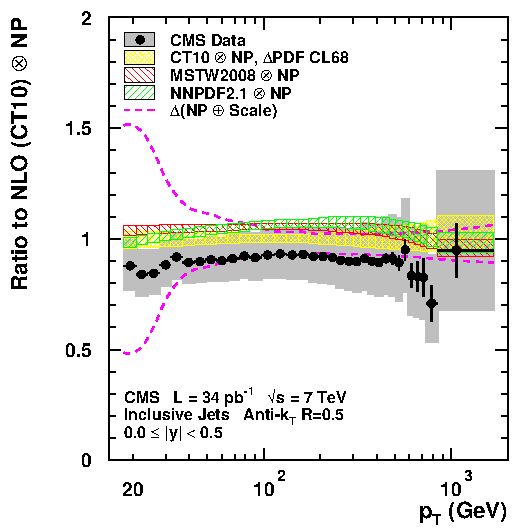
\includegraphics[width=0.43\textwidth]{fnl2342b_pdfcomp1_bin1.pdf}\hftwo%
  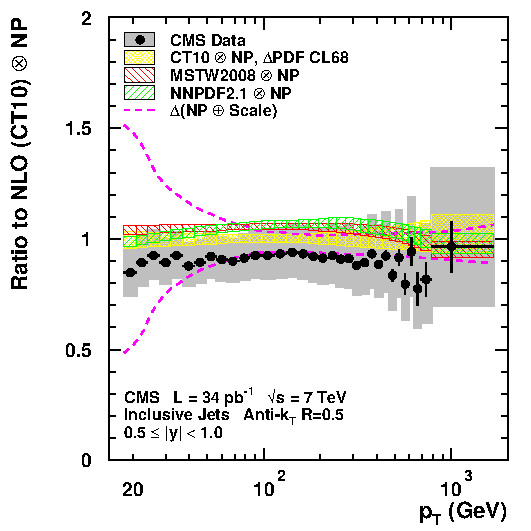
\includegraphics[width=0.43\textwidth]{fnl2342b_pdfcomp1_bin2.pdf}
  % 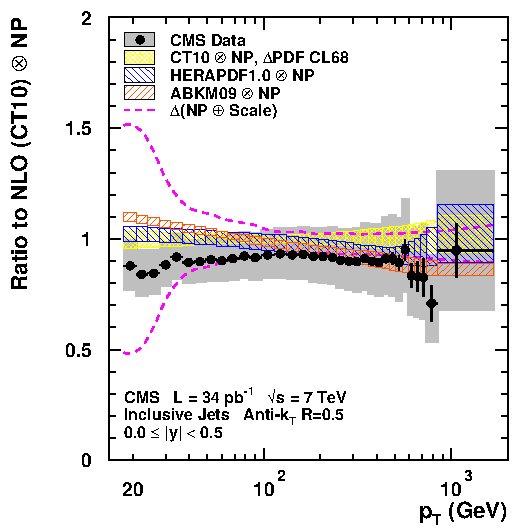
\includegraphics[width=0.43\textwidth]{fnl2342b_pdfcomp2_bin1.pdf}\hftwo%
  % 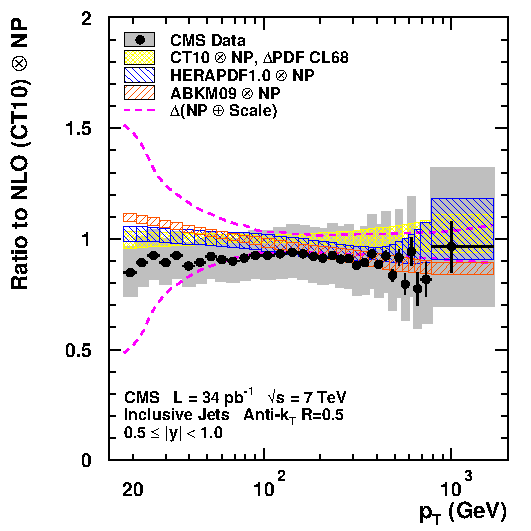
\includegraphics[width=0.43\textwidth]{fnl2342b_pdfcomp2_bin2.pdf}
  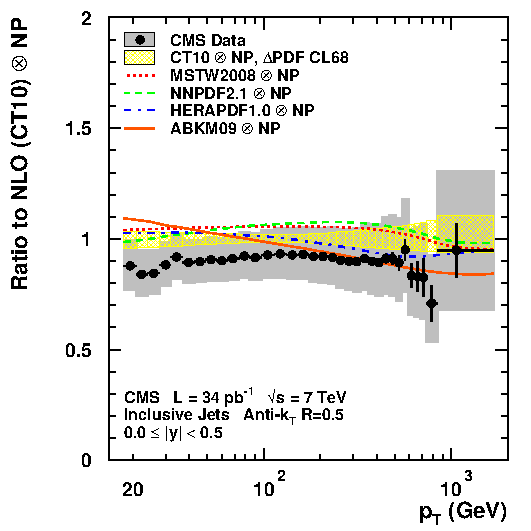
\includegraphics[width=0.43\textwidth]{fnl2342b_pdfcomp3_bin1.pdf}\hftwo%
  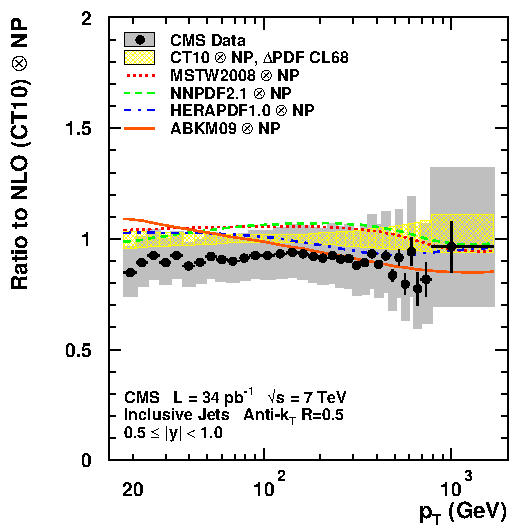
\includegraphics[width=0.43\textwidth]{fnl2342b_pdfcomp3_bin2.pdf}
  \caption{CMS inclusive jet data for $|y| < 0.5$ (left) and $0.5 \leq
    |y| < 1.0$ (right) are presented vs.\ $p_{\mathrm{T}}$ with
    statistical (error bars) as well as systematic uncertainties (grey
    band) as ratio to NLO using the CT10 PDFs. Additional predictions
%    are shown using the MSTW2008 and NNPDF2.1 (top) or the HERAPDF1.0
%    and ABKM09 PDFs (middle). PDF uncertainties are displayed as
    are shown using the MSTW2008 and NNPDF2.1 PDFs (top). PDF
    uncertainties are displayed as colored bands. The central results
    of four additional PDFs are also shown together as lines in one
    plot (bottom).  Common theoretical uncertainties from scale
    choices and NP corrections are indicated by dashed magenta lines
    (top and middle).}
  \label{fig:InclJetsBins12}
\end{figure}

%%%%%%%%%%%%%%%%%%%%%%%%%%%%%%%%%%%%%%%%%%%%%%%%%%%%%%%%%%%%%%%%%%%%%%%%%%%%%%%

\clearpage \bibliographystyle{lucas_unsrt} %
\bibliography{fnlotut}

\end{document}
